\newpage
%%%%%%%%%%%%%%%%%%%%%%%%%%%%%%%%%%%%%%%%%%%%%%%%%%%%%%%%%%%%%%%%
%%%%%%%%%%%%%%%%%%%%%%%%%%%%%%%%%%%%%%%%%%%%%%%%%%%%%%%%%%%%%%%%
%%%%%%%%%%%%%%%%%%%%%%%%%% Enunciado %%%%%%%%%%%%%%%%%%%%%%%%%%%

\begin{myblock}
\phantomsection\addcontentsline{toc}{section}{Ejercicio \#5 | Curvas ROC/AUC}
\section*{Ejercicio \#5 | Curvas ROC/AUC}

Construyan la curva ROC para el problema de daño coronario y su relación con la edad visto en la
clase 3 del curso. 

\end{myblock}

%%%%%%%%%%%%%%%%%%%%%%%%%%%%%%%%%%%%%%%%%%%%%%%%%%%%%%%%%%%%%%%%
%%%%%%%%%%%%%%%%%%%%%%%%%%%%%%%%%%%%%%%%%%%%%%%%%%%%%%%%%%%%%%%%

\subsection{Teoría}

    \subsubsection{Especificidad y Sensibilidad}

        Las curvas ROC, del acrónimo en inglés ``\textit{Receiver Operating Characteristic}'', es una herramienta
        bastante útil para la evaluación de clasificadores. Formalmente, dado un clasificador que produce scores
        continuos $S \in \mathbb{R}$, la curva ROC representa el conjunto de pares $(FPR(t), TPR(t))$ para
        todo $t \in \mathbb{R}$, donde $t$ es un umbral de decisión.

        Matemáticamente hablando, para una variable aleatoria continua $X$ que representa los scores y una variable
        indicadora $Y \in \{0,1\}$, que representa la clase verdadera, tenemos:

        \begin{itemize}
            \item $TPR(t) = P(X > t | Y = 1) = 1 - F_1(t)$
            \item $FPR(t) = P(X > t | Y = 0) = 1 - F_0(t)$
        \end{itemize}

        Donde $F_1$ y $F_0$ son las funciones de distribución acumulada condicionales de $X$ dado $Y = 1$ y
        $Y = 0$, respectivamente.  

        Ahora bien, el AUC, o Área Bajo la Curva, posee una elegante interpretación probabilística que fundamenta
        su utilidad como medida de desempeño: $\text{AUC} = P(S^+ > S^-)$. En este caso, $S^+$ y $S^-$ son scores
        independientes correspondientes a observaciones positivas y negativas, respectivamente. Esta formulación
        establece que el AUC equivale a la probabilidad de que el clasificador asigne un score mayor a una observación
        positiva elegida aleatoriamente que a una negativa aleatoriamente. 

        Hablando de los ejes, el Eje X se refiere a los \textit{False Positive Rate}, o FPR:

        \[
            \text{FPR} = \frac{\text{FP}}{\text{FP + TN}} = 1 - \text{Especificidad}
        \]

        Este eje representa la fracción de negativos que el modelo clasifica erróneamente como positivos. 

        En cuanto al eje Y, se trata del \textit{True Positive Rate} o TPR, y se define como:

        \[
            \text{TPR} = \frac{\text{TP}}{\text{TP + FN}} = \text{Sensibilidad}
        \]

        Representa la fracción de positivos correctamente identificados por el modelo. 

        Creo que es importante recordar lo que son Sensibilidad y Especificidad. La sensibilidad o \textit{recall}, 
        es una métrica que se encarga de medir la capacidad delk modelo para identificar correctamente los verdaderos
        positivos. Es fundamental en contextos donde los falsos negativos son costosos, como en aplicaciones de medicina
        o algo del apartado legal. En cuanto a la Especificidad, esta mide la capacida ddel modelo de identificar
        de manera correcta los verdaderos negativo. Es de vital importancia para cuando los falsos positivos 
        son costosos, quizás para la aprobación de créditos. 

        De ese modo, cada punto de la curva representa un posible umbral de decisión. Cuando el umbrla es
        muy bajo, el modelo es demasiado flexible y clasifica en su mayoría como positivo, i.e. cuando TPR y FPR son altos.
        Cuando el umbral es muy alto, el modelo es muy rígido y clasidica casi todo como negativo, Esto es cuando TPR y FPR son bajos. 

        La recta que cruza por la identidad en las curvas ROC es la ``línea del azar''. La línea diagonal que
        une (0,0) con (1,1) corresponde a lo que sería un clasificador aleatorio, uno sin la capacidad de discernir. Cuando
        el modelo está sobr esta línea, entonces su desempeño no se puede distinguir del azar. Cuanto ms arriba 
        de la línea se encuentre la curva, mejor será la discriminación.

        Una de las desventajas de la curva ROC es que no es sensible al desbalance de clases. Para cuando hay
        prevalencia de desbalanceo de clases, se prefiere utilizar la curva \textit{Precision-Recall} (PR). Para
        la evaluación de modelos, la ROC es bastante útil para comparar de forma global.

    \subsubsection{Estadístico de Youden}

        El estadístico de Youden, también conocido como índice J, fue introducido en 1950 por W.J. Youden como
        una medida resumen de la efectividad de una prueba diagnóstica. Se define como:

        \[
            J = \text{Sensibilidad} + \text{Especificidad} - 1
        \]

        El rango del índice es, naturalemnte, $-1 \leq J \leq 1$. Sin embargo, en aplicaciones prácticas, 
        se acota a $0 \leq J \leq 1$, ya que la sensibilidad y especificidad son no negativas. En el caso de
        la curva ROC, tenemos que la Sensibilidad es TPR y que 1 - Especificidad es FPR. Entonces:

        \[
            J = TPR - FPR
        \]

        Por lo tanto, $J$ mide la distancia vertical máxima entre la curva ROC y la diagonal de azar.

        \begin{itemize}
            \item $J = 0$ el modelo no discrimina, i.e. estaríamos hablando a un clasificador aleatorio.
            \item $J = 1$ el modelo clasifica de manera perfecta, i.e. la sensibilidad y especificidad son ambos 1.
            \item Valore sintermedios reflejan la capacidad de la prueba de mejorar sobre el azar. 
        \end{itemize}

        Cuando un modelo produce un puntaje o probabilidad, se necesit aun umbral de decisión para clasificar. El
        umbral óptimo de Youden se define como aquel que maximiza $J$:

        \[
            \hat{t} = \text{arg} \max_t \bigg(\text{Sensibilidad}(t) + \text{Especificidad}(t) - 1\bigg)
        \]

        Este pubnto corresponde al punto de la curva ROC más alejado de la diagonal del azar. 

    \subsubsection{Estadístico Kolmogorov-Smirnov (KS)}

    Este estadístico proviene originalmente de la prueba KS para comparar dos distribuciones acumuladas. En
    su forma general:

    \[
        D = \sup_x |F_n(x) - F(x)|
    \]

    Es la máxima diferencia entre una función de distribución empírica y una distribución teórica. En
    clasificación binaria, se adapta para medir la separación enter las distribuciones de puntajes (o probabilidades)
    de las dos clases. 

    La interpretación probabilística del KS mide cuán bien el modelo separa las distribuciones de scores
    entre positivos y negativos. Geométricamente, se demuestra que:

    \[
        KS = \max_t |TPR(t) - FPR(t)|
    \]

    Donde $t$ es un umbral de decisión. Es decir, $KS$ es la máxima diferencia vertical entre la curva ROC
    y la diagonal de azar. Esto es identico al de Youden solo cuando $TPR \geq FPR$. 

    \begin{itemize}
        \item KS = 0 nos dice que no hay discriminación, las distribuciones son idénticas.
        \item KS = 1 nos dice que la separación es perfecta, sin solapamientos entre positivos y negativos.
        \item Los valores intermedios reflejan distintos niveles de discriminación.
    \end{itemize}

\subsubsection{Distancia al punto (0,1)}

En el espacio ROC, el punto ideal para un clasificador perfecto es (0,1), pues se traduce en FPR = 0, i.e. ningún
falso positivo, y TPR = 1, i.e. todos los positivos identificados correctamente. Minimizar la distancia a 
ese punto significa encontrar el mejor compromiso entre reducir los falsos positivos y aumentar los verdaderos positivos. A 
diferencia del índice Youden, este midel al distancia euclidiana absoluta ideal. 


%%%%%%%%%%%%%%%%%%%%%%%%%%%%%%%%%%%%%%%%%%%%%%%%%%%%%%%%%%%%%%%%
%%%%%%%%%%%%%%%%%%%%%%%%%%%%%%%%%%%%%%%%%%%%%%%%%%%%%%%%%%%%%%%%

\subsection{Resultados}
\textcolor{red}{
En este caso, grafiqué dos curvas ROC. Al final me di cuenta de que fue redundante, porque este tipo de visualizaciones para problemas de clasificación binaria no necesitan mostrar
la aproximación cuando se toma a 1 o a 0 como la clase positiva. Obtener los dos gráficos y obtener
sus estadísticos es redundante. Sin embargo se ven bonitas las gráficas.}
\clearpage

    \subsubsection{Estadístico de Youden \& Kolmogorov-Smirnov}

        \begin{figure}[h!]
            \centering
            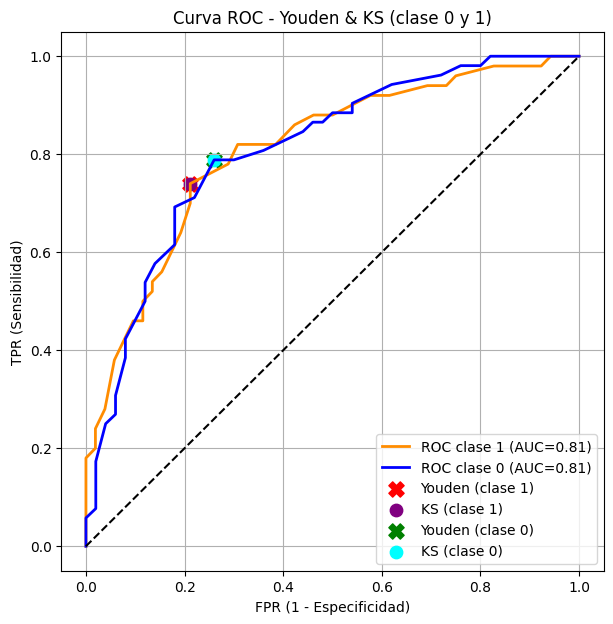
\includegraphics[width=0.7\linewidth]{Images/youden-ks-roc.png}
            \caption{Curva AUC/ROC con los estadísticos de Youden \& KS fijos en el mismo lugar.}
            \label{fig:youden-ks-roc}
        \end{figure}
        \clearpage

    \subsubsection{Punto (0,1) geométrico.}

        \begin{figure}[h!]
            \centering
            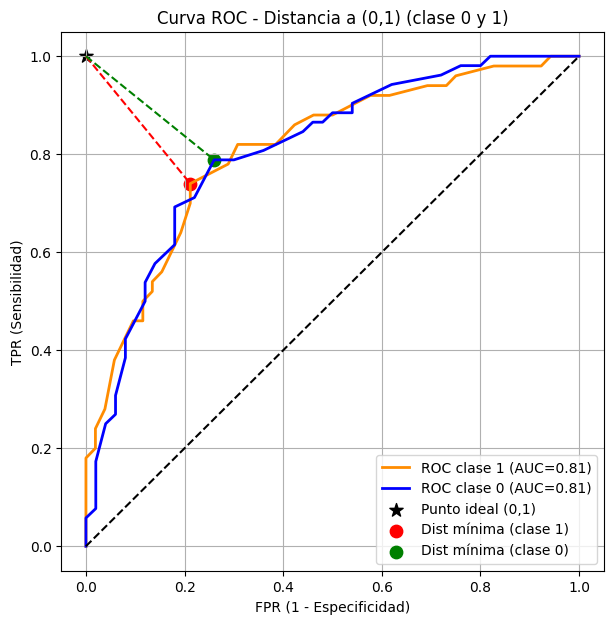
\includegraphics[width=0.7\linewidth]{Images/dist-geom-roc.png}
            \caption{Curva AUC/ROC con los estadísticos geométricos en el mismo lugar que el de Youden \& KS.}
            \label{fig:geom-roc}
        \end{figure}

    \subsubsection{Discusión de resultados}

        Para nuestro caso, nos encontramos con que el estadístico de Youden, el de Kolmogorov-Smirnov y 
        la distancia del máximo de la ROC hacia el punto (0,1) coinciden por completo. Es decir, existe
        un punto óptimo único dentro de la curva, de tal modo que se maximiza la capacidad del modelo 
        bajo el mismo umbral. 

        Recordemos que el índice de Youden maximiza la suma de la sensibilidad y especificidad. Esto es,
        equivale a cuando encontramos el punto donde la diferencia entre la tasa de verdaderos positivos, y la
        de falsos positivos es máxima, i.e. el punto más alejado de la recta del azar. El estadístico de
        KS maximiza la separación entre las distribuciones de scores de las clases positiva y negativa. En
        cuanto a la distancia al punto (0,1), este minimiza la distancia euclidiana al punto ideal donde TPR = 1 
        y FPR = 0, mientras más bajo el valor, más cerca de la mejor clasificación está nuestro modelo. 

        Que los puntos coincidan nos está diciendo que existe un punto de operación óptimo. Entonces tenemos
        un umbrla que ofrece un rendimiento consistente y robusto. A pesar de que graficamos dos ROC, una para
        cuando la clase 1 es positiva y otra para cuando la 0 es positiva (redundante por ser un clasificador
        biomial), concentremonos en la clase 1 como la positiva. Cuando clase 1 es positiva, el umbral óptimo está en 0.524m con un accuracy de 0.765 y un F1-score de 
        0.755. 

        Finalmente, la coincidencia de estadísticos nos facilita la elección del umbral en la práctica, ya
        que no hay conflicto entre los criterios. Es importante recordar que el umbral es un valor que nos 
        permite configurar qué tan flexible será nuestro modelo. Por ejemplo, si la probabilidad < umbral, entonces
        se toma como clase negativa, si la probabilidad es $/geq$ umbral, entonces tomamos clase positiva.
        
        Si hacemo suna analogía, un umbral de 0.3, dejamos que varios falsos positivos sean clasificados de manera
        incorrecta. Si tomamos un umbral de 0.8, dejamos que algunos verdaderos positivos sean mal clasificados. 
        

%%%%%%%%%%%%%%%%%%%%%%%%%%%%%%%%%%%%%%%%%%%%%%%%%%%%%%%%%%%%%%%%
%%%%%%%%%%%%%%%%%%%%%%%%%%%%%%%%%%%%%%%%%%%%%%%%%%%%%%%%%%%%%%%%

\subsection{Código}

    \begin{lstlisting}[caption={Analisis de Curva ROC para Clasificacion Logistica}, label={lst:roc_analysis_py}]
    # --- Ajuste del modelo y funcion auxiliar ---
    # Modelo logistico
    logit = LogisticRegression(solver="lbfgs")
    logit.fit(edad.reshape(-1, 1), coro)
    phat = logit.predict_proba(X)[:, 1] # Probabilidad de la clase 1

    # Funcion que calcula metricas ROC y puntos de corte optimos
    def compute_metrics(y_true, scores, positive_label=1):
        if positive_label == 0: # Invierte para analizar la clase 0
            y_true, scores = 1 - y_true, 1 - scores

        fpr, tpr, thresholds = roc_curve(y_true, scores)
        roc_auc = auc(fpr, tpr)

        # Puntos de corte optimos
        youden_idx = np.argmax(tpr - fpr)
        ks_idx = np.argmax(np.abs(tpr - fpr))
        dist_idx = np.argmin(np.sqrt(fpr**2 + (tpr - 1)**2))

        # Resultados en puntos optimos
        results = {}
        for name, thr in [("Youden", thresholds[youden_idx]),
                        ("KS", thresholds[ks_idx]),
                        ("Dist", thresholds[dist_idx])]:
            y_pred = (scores >= thr).astype(int)
            acc = accuracy_score(y_true, y_pred)
            f1 = f1_score(y_true, y_pred)
            results[name] = (thr, acc, f1)

        return fpr, tpr, roc_auc, youden_idx, ks_idx, dist_idx, results

    # --- Calculo y visualizacion ---
    # Metricas para ambas clases
    fpr1, tpr1, auc1, y_idx1, ks_idx1, d_idx1, res1 = compute_metrics(y, phat, 1)
    fpr0, tpr0, auc0, y_idx0, ks_idx0, d_idx0, res0 = compute_metrics(y, phat, 0)

    # Se grafica con matplotlib

    # Imprimimos metricas
    \end{lstlisting}


\subsection{Resumen de codigo}

\begin{itemize}
    \item \textbf{Modelo y Predicciones:} Se ajusta un modelo de regresion logistica utilizando la edad como predictor. Posteriormente, se calculan las probabilidades predichas (\texttt{phat}) para la clase positiva (1).

    \item \textbf{Funcion de Metricas:} Se define una funcion, \texttt{compute\_metrics}, que es el nucleo del analisis. Esta funcion calcula la curva ROC y el area bajo la curva (AUC). Ademas, identifica los umbrales de decision optimos basados en tres criterios distintos:
    \begin{itemize}
        \item El indice de Youden (maximizando la diferencia TPR - FPR).
        \item La estadistica de Kolmogorov-Smirnov (KS) (maximizando la diferencia absoluta |TPR - FPR|).
        \item La distancia minima al punto ideal (0,1) en el grafico ROC.
    \end{itemize}
    Para cada umbral optimo, la funcion tambien calcula la exactitud (accuracy) y la puntuacion F1.

    \item \textbf{Analisis por Clase:} La funcion de metricas se aplica dos veces para evaluar el rendimiento del clasificador tanto para la clase 1 (positiva) como para la clase 0 (negativa). Para la clase 0, se invierten las etiquetas y las probabilidades.

    \item \textbf{Visualizacion:} Se generan dos graficos de la curva ROC para comparar el rendimiento de ambas clases. El primer grafico resalta los puntos optimos segun Youden y KS, mientras que el segundo resalta el punto optimo basado en la distancia minima a (0,1).

    \item \textbf{Reporte:} Finalmente, se imprime un resumen en la consola que muestra el valor del umbral, la exactitud y la puntuacion F1 para cada uno de los tres criterios de optimizacion, detallando los resultados para ambas clases.
\end{itemize}

%%%%%%%%%%%%%%%%%%%%%%%%%%%%%%%%%%%%%%%%%%%%%%%%%%%%%%%%%%%%%%%%
%%%%%%%%%%%%%%%%%%%%%%%%%%%%%%%%%%%%%%%%%%%%%%%%%%%%%%%%%%%%%%%%

%\subsection{Conclusiones}

%%%%%%%%%%%%%%%%%%%%%%%%%%%%%%%%%%%%%%%%%%%%%%%%%%%%%%%%%%%%%%%%
%%%%%%%%%%%%%%%%%%%%%%%%%%%%%%%%%%%%%%%%%%%%%%%%%%%%%%%%%%%%%%%%

\clearpage




